\documentclass[12pt]{article}
\author{Maedeh Karkhaneh Yousefi}
\title{HomeWork4}
\usepackage{graphicx}
\usepackage{float}
\usepackage{subcaption}
\begin{document}
\maketitle
I first used LabelEncoder and MinMaxScaler to prepare the data. Then used the 'age', 'sex', 'bmi', 'children', 'smoker', 'region' as features and 'charges' as target. 
I found the best structure is having 4 Denses, each having 8, 16, 16, 32 and 1 units, respectively, with 100 epochs and 32 as batch-size; Otherwise, over-fitting would be seen from the loss-epochs and mae-epochs plots. 
\begin{figure}[H]
\centering
\begin{subfigure}{0.5\linewidth}
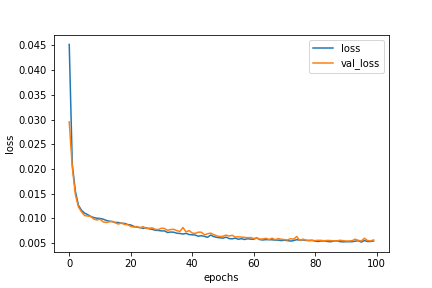
\includegraphics[width=\textwidth]{loss.png}
\end{subfigure}
\begin{subfigure}{0.5\linewidth}
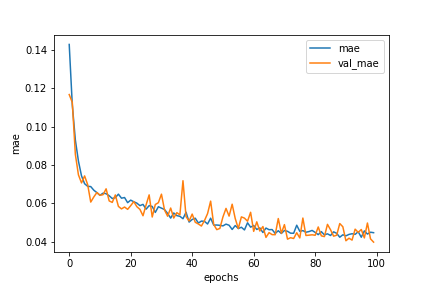
\includegraphics[width=\textwidth]{mae.png}
\end{subfigure}
\label{mesh:fig1}
\caption{Model's loss and mae plot.}
\end{figure}
\pagebreak
Then I transformed the input data by using Polynomial Features. 
\begin{figure}[H]
\centering
\begin{subfigure}{0.5\linewidth}
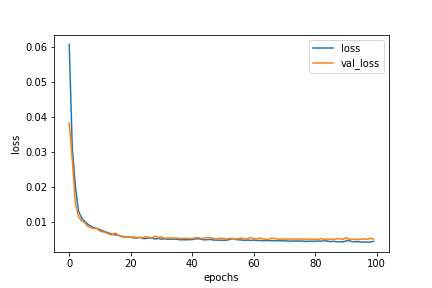
\includegraphics[width=\textwidth]{loss_poly.png}
\end{subfigure}
\begin{subfigure}{0.5\linewidth}
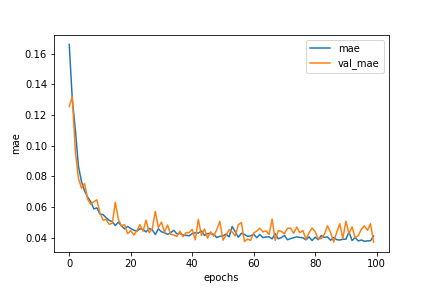
\includegraphics[width=\textwidth]{mae_poly.png}
\end{subfigure}
\label{mesh:fig1}
\caption{Model's loss and mae plot using Polynomial Features.}
\end{figure}
\end{document}